\documentclass[conference]{IEEEtran}
\IEEEoverridecommandlockouts
% The preceding line is only needed to identify funding in the first footnote. If that is unneeded, please comment it out.
\usepackage{cite}
\usepackage{amsmath,amssymb,amsfonts}
\usepackage[hidelinks]{hyperref}
\usepackage{algorithmic}
\usepackage{graphicx}
\usepackage{booktabs}
\usepackage{textcomp}
\usepackage{xcolor}

\def\BibTeX{{\rm B\kern-.05em{\sc i\kern-.025em b}\kern-.08em
    T\kern-.1667em\lower.7ex\hbox{E}\kern-.125emX}}
\begin{document}


\title{Composition of concrete and its influence on compressive strength\\
%{\footnotesize \textsuperscript{*}Note: Sub-titles are not captured in Xplore and
%should not be used}
%\thanks{Identify applicable funding agency here. If none, delete this.}
}

\author{\IEEEauthorblockN{Filipe P. de Farias}
\IEEEauthorblockA{\textit{Department of Teleinformatics Engineering} \\
\textit{Federal University of Ceará}\\
Fortaleza, Brazil \\
filipepfarias@fisica.ufc.br}
\and
\IEEEauthorblockN{Yvo J. M. Sales}
\IEEEauthorblockA{\textit{Department of Teleinformatics Engineering} \\
\textit{Federal University of Ceará}\\
Fortaleza, Brazil \\
yvo@gtel.ufc.br}
}

\maketitle

\begin{abstract}
The compressive strength of a concrete is a important property since it impacts directly on its applications. The classical approach to obtain the compressive strength of a specific concrete mixture is to submit a sample to a test on a hydraulic press. However, it takes time to perform this type of test since it is necessary to wait the sample to cure. In this work, we try to find a regression model to accurately estimate the compressive strength of a concrete mixture from the concentration of its components.
\end{abstract}

\begin{IEEEkeywords}
Regression models, concrete compressive strength, machine-learning, partial least squares.
\end{IEEEkeywords}

\section{Introduction}
A material formed by aggregates bonded together by a fluid material that hardens over time has been used by humans for construction since many years ago~\cite{b3}. Nowadays this material is known as concrete and it's widely used in the construction field. The aggregates used in the mixture of the concrete affect directly its compressive strength which highly impacts its applications. For instance, in general, the concrete for columns or beams needs to have a greater compressive strength than the one for pavement. On the previous work, we have made a statistical analysis on a dataset extracted from the UCI Machine Learning Repository (University of California, Irvine)~\cite{b4} that collects information about the concentration of some aggregates used to form different mixtures of concretes. In this work, we try to find a regression model to estimate the relation between the concentration of those aggregates and the strength of the concrete mixture. The goal is that such model could be a good replacement to tests of samples on hydraulic press.

This work is divided as follows. A description of the data is given in Section~\ref{sec:data_description} resulted from the previous work with the addition of the regressor (concrete compressive strength). Section~\ref{sec:rm} brings a brief introduction to the regression models that will be used to fit the data. In the sequel, we present and discuss the results in Section~\ref{sec:results}. Finally, the conclusions and considerations are exposed in Section~\ref{sec:conclusions}.

% This works tries to predict this compressive strength and to classify when the concrete is proper to be applied in structures.  In the UCI database the concrete is tested with different components concentrations and different curing time (ages). 

\section{Data description}\label{sec:data_description}

The composition of each one of the $N$ = 1030 concrete samples is given by the concentrations (kg/m\textsuperscript{3}) of $D$ components: Cement, Blast Furnace Slag, Fly Ash, Water, Superplasticizer, Coarse Aggregate and Fine Aggregate, as summarized in Table~\ref{data_description_table}. 
%
The cement is what binds the elements of the concrete together. 
%
Indeed his technical name in the literature is \emph{binder}~\cite{b5}. 
%
The other components as blast furnace slag and fly ash, the outcomes of another industrial process reused in the concrete mixture, they have the role of increase the chemical hardness of the concrete, i.e. in a microscopic level. 
%
The water is responsible for react with the cement resulting in the cement stone. 
%
The superplasticizer gives fluid characteristics to the concrete aiming to better fill the mold and decrease the use of water. 
%
The coarse and fine aggregates give some macroscopical mechanical resistance to the concrete but can reduce its compressive strength if bad applied. 
%
Their major role is to occupy the spaces in the mold reducing the use of cement. 
%
The output is the concrete compressive strength which is measure in the stress test where a force its applied to a sample using a hydraulic press. 
%
When the sample reaches the rupture point, the pressure, force per area of the sample, is observed. 

\begin{table}[htp]
\caption{Data description}
\begin{center}
  \begin{tabular}{@{} clc @{}}
    \toprule
    Label & Component & Unit \\ 
    \midrule
    $D_1$ & Cement & kg/m\textsuperscript{3} \\ 
    $D_2$ & Blast Furnace Slag & kg/m\textsuperscript{3} \\ 
    $D_3$ & Fly Ash & kg/m\textsuperscript{3} \\ 
    $D_4$ & Water & kg/m\textsuperscript{3} \\ 
    $D_5$ & Superplasticizer & kg/m\textsuperscript{3} \\ 
    $D_6$ & Coarse Aggregate & kg/m\textsuperscript{3} \\ 
    $D_7$ & Fine Aggregate & kg/m\textsuperscript{3} \\ 
    $D_8$ & Age & days \\ 
    ${\bf D_9}$ & {\bf Compressive strength} & {\bf MPa} \\ 
	\midrule
    Total & $N=$ 1030 samples&  \\ 
    \bottomrule
  \end{tabular}
\end{center}
\label{data_description_table}
\end{table}%

The concrete mixtures were divided into a set $\mathcal{L} = \{L_1\,, L_2\,, L_3\}$ of classes~\cite{b1} based on their compressive strength, following the function $\mathcal{C} \colon \mathcal{R} \mapsto \mathcal{L}$ defined in Eq.~\ref{eq:labeling_function}. The mixture which is weak and not recommended for structures, the \emph{Non-standard}, was labeled with $L_1$ and comprises 295 samples. The mixture whose strength is in a range that can be applied to structures is classified as $L_2$, or \emph{Standard}, and comprises 525 samples. The high performance mixture $L_3$, \emph{High-strength} and comprises 210 samples.
%
\begin{equation}\label{eq:labeling_function}
  \mathcal{C}(D_9) = \begin{cases}
    L_1\,, D_9 < 25\\
    L_2\,, 25 \leq D_9 < 50\\
    L_3\,, D_9 \geq 50
  \end{cases}
\end{equation}
%
where $D_9$ is the compressive strength of the concrete mixture.

The observations are the measured compressive strengths of each sample and, as the predictors $D_1 - D_7$, are real valued. The Age ($D_8$) of the concrete is extremely discrete. All the data was normalised, by centering at the mean and scaling by the standard deviation to avoid any of the methods to be sensitive to different scales. At Fig. \ref{histogram_biplot} we note the strongest positive correlation is between the strength and the cement component ($D_9 \times D_1$). Another important factors are the presence of the superplasticizer ($D_9 \times D_5$) and the age that represents the time of cure ($D_9 \times D_8$). In all these components is noted a subtle correlation. And the most important fact that can be observed is the decrease of the necessity of water when the superplasticizer is used ($D_5 \times D_4$), which was its proposal in the first place.
\begin{figure}[htbp]
\centerline{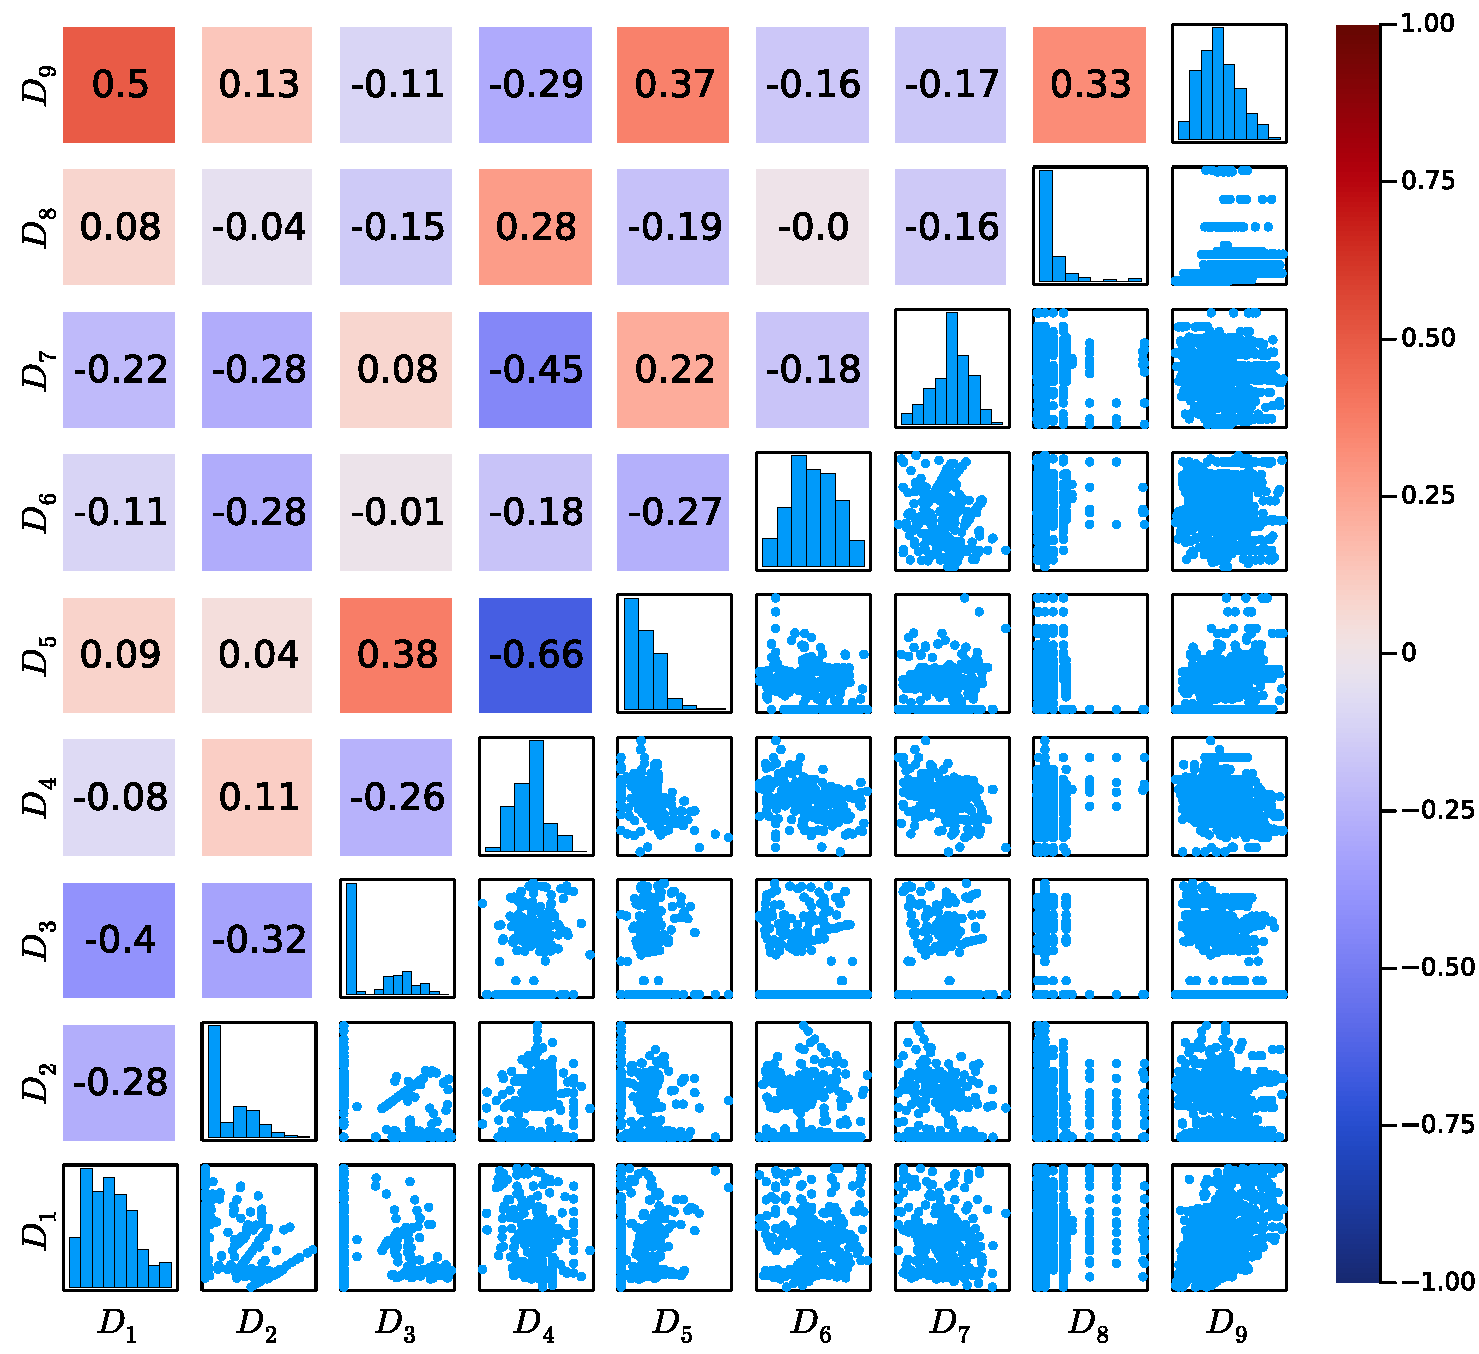
\includegraphics[width=\columnwidth]{../figures/correlation_predictors_outcomes}}
\caption{Pairwise scatter, correlation and histogram plots of each concrete component.}
\label{histogram_biplot}
\end{figure}

\section{Regression models}\label{sec:rm}

Regression models try to find relations between the \emph{independent variables} and the \emph{dependent variables}, which are named, respectively, predictors and outcomes in this work. These relations can occur in different forms. The simplest one is the linear relationship, which is when the curve predictors \textit{vs} outcomes, in the case that both are one-dimensional, forms a simple line and, in the general case, a hyperplane. Continuing the discussion of the last work, we now change the strategy to use a non-linear method for regression, in this case using neural networks.

\subsection{Neural networks regression}

In this method, expressed in Eq.\ref{eq:nn-reg}, each predictor $x_k$ is weighted by a real-valued constant $w_k$. The outcome is inputed in an activation function $\phi$ which will be ``activated'' when that sum be enough to reach a given output $Y$. This output will be the data, specifically the value of the compressive strength.

\begin{equation}\label{eq:nn-reg}
Y = \phi \left( \sum_k w_k \cdot x_k \right)
\end{equation}

The shape of $\phi$ is a choose of the one who is modelling. Some of them are the sigmoid and the step functions. In this work, the ReLU function was used, which is defined as 

\begin{equation}
\phi_\text{ReLU}(x) = \operatorname{max}(0,x).
\end{equation}

The next step, which is to optimise a cost function is quite similar to the ordinary linear squares, but now observing that the function is different, but yet the cost will be defined as the distance between the data and the values of the model.

\section{Classification models}
The regression models are used to fit output variables that are quantitative. But, in the majority of the applications, the output variables are qualitative instead, which means that classification models must be used to fit those variables. The classification models estimate the probability of the outcome $Y$ to belong to a class $L$ given a set of predictors $X$, i.e. the probability $Pr(Y=L|X)$.

In this section, we briefly describe the classification models that were used throughout this paper.

\subsection{Linear discriminant analysis}
The linear discriminant analysis models the probability distribution of the predictors for each one of the outcome classes and applies the Bayes' theorem to them in order to estimate the probabilities $Pr(Y=L | X=x)$, which is the probability of the outcome $Y$ to belong to the class $L$ given that the predictors $X$ assume a value $x$. Let $\pi_L$ be the prior probability of a random chosen sample to belong to the class $L$ and $f_L(x) = Pr(X=x, Y=L)$ denote the probability density function of $x$ given that a sample belongs to the class $L$, then the Bayes' theorem states that

\begin{equation}
  Pr(Y=L | X=x) = \frac{\pi_L f_L(x)}{\sum_{i = 1}^{|\mathcal{L}|}\,. \pi_i f_i(x)}
\end{equation}

\subsection{Neural networks}

\subsection{Nearest neighbors}

\subsection{Support vector classifier}

\section{Results} \label{sec:results}

\section{Conclusions}\label{sec:conclusions}

The database of concrete is not easy to analyse if there is no previous knowledge about the problem of the components mixture, as was noticed in the previous work and a more deep literature research was needed. Although the models worked, the authors were not capable to determine if the errors found imply in safe conditions for the concrete, neither is the objective of this work. What we can conclude is that the model is not linear given the $R^2$ statistics and the original work of the data~\cite{b4}.
%In none of the analysis the data have been shown as separable on the initially determined classes. The next step is to try to perform regression to model the compressive strength itself before trying to classify the samples. in the literature \cite{b6} is more common an analysis of the concrete data stratified by the Age, what was not done in this work and maybe the cause of poor correlations.

\begin{thebibliography}{00}
\bibitem{b1} ACI Manual of Concrete Practice 2000, Part 1: Materials and General Properties of Concrete.  American Concrete Institute.  Farmington Hills, MI.
\bibitem{b2} Tibshirani, Robert, et al. The Elements of  Statistical Learning:  Data Mining, Inference, and Prediction. Germany, Springer New York, 2009.
\bibitem{b3} Mindess, S., and Young, J.F. Concrete. Prentice-Hall, Inc., Englewood Cliffs, NJ, 1981.
\bibitem{b4} I-Cheng Yeh, ``Modeling of strength of high performance concrete using artificial neural networks," Cement and Concrete Research, Vol. 28, No. 12, pp. 1797-1808 (1998)
\bibitem{b6} I-Cheng Yeh, ``Prediction of Strength of Fly Ash and Slag Concrete By The Use of Artificial Neural Networks," Journal of the Chinese Institute of Civil and Hydraulic Engineering, Vol. 15, No. 4, pp. 659-663 (2003). 
\bibitem{b5} Khasanov, Irmuhamedova, et al, ``Theoretical foundations of the structure formation of cement stone
and concrete," IOP Conf. Series: Materials Science and Engineering 869 (2020)
\end{thebibliography}
\end{document}